%pdflatex-../thesis.tex
% vim:spell spelllang=en_us

% Networking
Networking is essential part of cloud computing because it would not be possible to access any services without networking. All services in cloud networking paradigm are accessed through data network. Network is also used for the communication between virtual machines, fo migrations, storage access and many other purposes.


% L1
Various Ethernet versions are used in cloud data centers. There are many versions with different link bandwidth and wiring, but 1G and 10G with twisted pairs or optical fibers are used most widely. Fast Ethernet were used in the past but it does not make sense to use it for server link today because bandwidth is limited to 100M and price is similar to Gigabit Ethernet.

% server
It is common to insert two independent \Ac{NIC}s into every server and connecting them into independent switches because it improves fault-tolerance. There is usually one more \Ac{NIC} for remote management. Remote management can be connected using detached cable or shared with any of network interfaces. Separate cable brings more flexibility and fault-tolerance, shared cable reduces cabling and simplifies maintenance. Both solutions are used. 

% rack & ToR
About 40 servers fit into traditional rack and these servers must be connected to network infrastructure. There are different topologies, but most common is hierarchical structure with two or three tiers. \cite{survey-architectures} There is also approach called \Uv{fabric} which implies non-blocking every-to-every mesh connection between switches. However, fabric technologies are proprietary and limited to the vendor. 
% možno doplnit a více ocitovat survey-architectures

Every rack can contain about 40 servers and these servers are connected to switch called \Ac{ToR}. This switch is located in the rack and acts as access layer for servers. Servers are connected to at least two \Ac{ToR}s if additional fault-tolerance is required. Upper network topology layers depends on data center size and scaling requirements. 
%There can be distribution and core layer, collapsed core or some kind of fabric.

%Physical topology must be adjusted to spread network layers between two or more datacenter networks. It is obviously not possible to spread physical layer, but data link layer and upper layers are possible to spread.

% L3 & address
Another view on network topology is network layer. Internet is based on \Ac{TCP}/\Ac{IP} so it is necessary to use this protocol family and assign \Ac{IP} addresses to servers, virtual machines and other network elements. There are two different versions of \Ac{IP} protocol:
\begin{description}
	\item[version 4] is the older version, with 32 bit address space. This version is still used more than version 6 even though it's address space is depleted and new version exists for more than 15 years.
	\item[version 6] is the \Uv{new} one, uses 128 bit address space and different headers, it is incompatible with version 4.
\end{description}

Modern data center must provide both versions of \Ac{IP} protocol because both versions are used.
However, there is a problem with obtaining public \Ac{IPv4} addresses because available pool is depleted. It is beneficial to employ \Ac{IPv6} protocol as primary one and try to limit the amount of required \Ac{IPv4} addresses.


There are different ways how to use both versions concurently:
\begin{itemize}
	\item Dual-stack is the simpliest and probably the most used way. One \Ac{IPv4} and one \Ac{IPv6} address is assigned to each interface. Use of both versions causes additional maintenance burden because it is necessary to manage two separate L3 networks.
	\item Tunelling \Ac{IPv6} via existing \Ac{IPv4} infrastructure with technologies like 6to4, 6rd or \Ac{ISATAP} is another way. This solution can be used for \Ac{IPv6} deployment in networks with working \Ac{IPv4}. 
	Tunelling is usually focused on deployment in access networks, but deployment in data center network is also applicable, as described in \cite{draft-sakura-6rd}.
	\item Translating \Ac{IPv4} addresses into \Ac{IPv6} addressing space is different approach than previous mentinoned because it operates on \Ac{IPv6}-only network. This technique does not require every box to have assigned an \Ac{IPv4} address and thus is good for saving address space. Hovewer address translations may not be suitable for data center usage because it does not preserve original \Ac{IP} addresses and makes customer tracking almost impossible. Further information can be found in \cite{ipv4-jako-sluzba}.
\end{itemize}

It is beneficial to deploy \Ac{IPv6} protocol as primary one in my opinion because it will become more and more needed over time. Hardware on current market usually supports protocol \Ac{IPv6} at least partialy, but there are still some hidden pitfalls. There may be problem for example with server's remote management that does not have to support \Ac{IPv6} protocol and thus it is totally unusable on \Ac{IPv6}-only network. None of the servers I have used for practical part of this thesis support remote management over \Ac{IPv6}. 
However, there is currently only small demand for \Ac{IPv6} support and \Ac{IPv6} deployment does not bring any direct benefit. Even thought there are many problems and advantages are invisible in short-term view, it is not possible to ignore this protocol.

Virtual machine migration must be taken into account durring addressing schema design because it plays crucial role in data center operation. Migrations are performed between hypervisors, i.e. physical servers, and these servers may be located in different racks, halls or even in different data centers. It is usually required to preserve \Ac{IP} address of virtual machine during migration process and thus adressing schema must be prepared to move single \Ac{IP} address around almost whole data center without any significant configuration changes. 

% shared L2
First solution for unlimited migrations while preserving \Ac{IP} address is L2 sharing between hypervisors. Data link layer is shared between all hypervisors and then virtual machine is located in the same L2 network before and after migration. This solution does not scale well since it is not recommended to place more than a few hundreds of hosts into a single L2 domain, necessitating division of single L2 into many smaller networks. This can be easily deployed for hypervisors in same rack, but it is more difficult to do with more distant servers and even more when servers are located at different data centers.

% routing 
Another way how to accomplish unlimited \Ac{VM} migrations is to use routing for machine connectivity. This method uses temporary and fixed \Ac{IP} addresses. Hypervisors do not have to be in same L2 network and there is higher variability in addresses assigned to virtual machines. Temporary address is assigned according to \Ac{VM}'s location and it changes during migration. Fixed address does not change during migration and packet with this destination address are routed to temporary address. Any routing protocol can be usel, e.g. \Ac{OSPF}, to provide correct routing of fixed address to the destination virtual machine. Is is neccesary to insert one record in routing table for every virtual machine because \textbackslash 32 routes are being advertised. Huge routing table may be problem for data centers with many virtual machines.

Higher layer is used to get more flexibility than lower level can offer. Main drawback of this solution is additinal complexity caused by routing and longer address swap because it takes some time to propagate routing to new temporary address. It is not easy to perform live migration because it is neccesary to change \Ac{IP} address of \Ac{VM}'s interface and thus opened sessions will terminate.

\subsection{Overlays}
\label{par:overlays}
Virtualization is heavily used these days, therefore it is necessary to provide networking solutions with at least same flexibility as virtualization offers. Multitenancy, \Ac{VM} migrations, fast reconfiguration and rapid deployment are most missing features of physical network. It is currently possible to migrate virtual machines without service interruption, but there is still not clear solution how to perform migration across whole data center with maintaining \Ac{IP} address. Overlay networking is one of the proposed solutions and it is supposed to bring additional abstraction layer capable of decoupling network from physical hardware. 
Technologies capable to build overlay network are \Ac{VXLAN}, \Ac{STT} and \Ac{NVGRE}. 

% STP
Data center network need to be robust so parallel paths are used to provide the redundancy and avoid outage caused by single link failure. It is necessary to avoid loops on L2 network but there are loops caused by redundant paths and L2 network does not use anything like \Ac{TTL} field.  Spanning Tree Protocol (\Ac{STP}) can be used to avoid loops in L2 networks, but there are two mayor problems. First is need to adjust \Ac{STP} if \Ac{VLAN}s are used because it is necessary to build special tree for each \Ac{VLAN}. Second problem caused by \Ac{STP} is utilization of parallel links. \Ac{STP} lefts only one of parallel link running and the others are disabled to avoid topology loops. It is suboptimal solution because links utilization is low and it is impossible to increase connection bandwidth by adding parallel links. Upgrading to higher link speed is limited and does not make economical sense. 10G cards are becoming affordable, but 40G cards are still very expensive.

% MAC table at ToRs
Servers housed in rack are usually connected to switch called Top of Rack (\Ac{ToR}) and this switch is learning \Ac{MAC} addresses. Common \Ac{ToR} switch have 24 or 48 ports so it should be able to learn addresses of these serves. However, virtualization techniques let us to run many virtual machines on single physical server so number of \Ac{MAC} addresses can increase significantly. Amount of addresses may grow even more because each virtual machine can have more than one interface and \Ac{ToR} switch must be able to learn all these addresses.

% Tenant isolation
Public cloud solutions tend to serve many tenants and it is necessary to avoid unwanted interaction between them. It is quite easy to guarantee this on virtualization layer but much harder to accomplish on network layer. Tenant isolation can be performed on Layer 3 or Layer 2. \Ac{VLAN}s are often used for isolation on Layer 2, but this solution suffer from insufficient scaling issues because only 12 bit \Ac{VLAN} identifier is used so it provides only 4096 different tags. This might be enough for smaller solution but it is not sufficient for huge cloud systems. Each physical server can host up to 100 virtual machines/containers\footnote{Server node2.brg/vpsfree.cz is currently running 117 \Ac{VPS}s with hardware: Supermicro \mbox{X9DR3-F}, 2x Xeon E5 2630Lv2, 256GB DDR3, 8x 2TB WD2002FAEX, 2x Intel DC S3700 200GB} owned by different tenants so 1 server can consume about 100 \Ac{VLAN} tags. All available tags can be depleted by 40 high performance servers which can fit in just one rack. Isolation at Layer 3 does not provide sufficient scaling as well. It is necessary to provide unlimited migration facility between hypervisors in different racks and it is sometimes is required to spread Layer 2 between all tenant's virtual machines. Layer 3 isolation is not capable of this.


%Some kind of encapsulation is usually used to build overlay network on top of physical network. Encapsulation of course have drawbacks in higher computation demand and packet size problems, but advantages brought by overlay are appreciable:
%\begin{itemize}
%	\item Configuration of physical network is left untouched, so configuration fails are minimized
%	\item Overlay network is only virtual and more flexible than physical network
%	\item It is easy to adjust overlay network since it is only done in software
%	\item Tenant isolation can be done better because overlays are designed to support this
%\end{itemize}

\subsubsection{VXLAN}
Virtual eXtensible Local Area Network is an overlay scheme with multitenancy and domain isolation. It is defined on Layer 3 and uses encapsulation as tunneling mechanism.

Most important thing is encapsulation since it provides \Ac{VXLAN} domain isolation and defines overlay network. Block called \Ac{VTEP} is responsible for encapsulation and tunnel organization. It analyzes every frame received from \Ac{VM} and prepend outer header with the label. This label is called \Ac{VXLAN} Network Identifier (\Ac{VNI}) and it is used to isolate domains. Virtual machines in different domains are not allowed to communicate directly with each other. Encapsulated packet is send to destination \Ac{VTEP} as an \Ac{UDP} packet. Destination \Ac{VTEP} unpacks packet, check whether there is any virtual machine in \Ac{VXLAN} domain and deliver the frame. \Ac{NVE} is another term for \Ac{VTEP} and it was used in \cite{rfc7365} as part of general network virtualization framework.

It is necessary for \Ac{VTEP} to be able to find destination \Ac{VTEP} for every encapsulated packet. This can be solved by data plane learning during forwarding as specified in \cite{rfc7348} or by acquiring this information from orchestrator. Getting information from orchestrator is better in my opinion because it avoids additional actions. Some kind of orchestrator or at least information system must be present in every data center and this system already knows location of all virtual machines as well as addresses of \Ac{VTEP}s. I think that it does not make sense to perform learning during forwarding because required informations are already saved in orchestrator. Orchestrator can directly distribute forwarding rules to all \Ac{VTEP}s or \Ac{VTEP} can ask orchestrator on-demand using any kind of \Ac{API}. Overlay unicast traffic can be forwarded directly to destination \Ac{VTEP} without any additional learning or even flooding.

% BUM traffic
There is traffic called \Ac{BUM} - Broadcast, Unknown unicast and Multicast which is not easy to handle by \Ac{VXLAN}. This kind of traffic needs to be delivered to more than one host in a single \Ac{VXLAN} domain and thus it is necessary to send encapsulated packet to many \Ac{VTEP}s at the same time. Multicast should be used as described in \cite{rfc7348}, but it requires mapping between \Ac{VXLAN} \Ac{VNI} and multicast address. This mapping should be managed by orchestrated. 
It would be beneficial to have technology for delivering \Ac{BUM} traffic without need of multicast because it brings additional complexity and it is not working in the global Internet. Unknown unicast can be mitigated with getting information about addresses from orchestrator as described in previous paragraph because the orchestrator knows all addresses and there is not any unknown traffic. 
Sending encapsulated broadcast and multicast to many \Ac{VTEP}s can be achieved by multicast in underlay network or any advanced delivery methods can be uses. It is possible to send this traffic as unicast between source \Ac{VTEP} and every other \Ac{VTEP}. However, this solution is suboptimal to packet duplication and higher network bandwidth usage. Only one advantages is that multicast in underlay network is not required. It is also possible to select on node as \Uv{router} for encapsulated \Ac{VXLAN} traffic between \Ac{VTEP}s but it is technically similar to building multicast tree and thus it might be easier to deploy multicast in underlay.
There is proprietary technology called IBM DOVE with is very similar to \Ac{VXLAN} but does not require multicast.

% network requirements

% VXLAN conclusion
I think that \Ac{VXLAN} is quite promising technology for network virtualization in data center. It brings much more flexibility that traditional \Ac{VLAN} approach and can be called as en evolution of \Ac{VLAN}. Principle of overlay network is building virtual network on the top of a physical infrastructure. Benefits were described in previous paragraphs and the main drawback is the lack of cooperation between overlay and underlay network. Multicast might be also quite problematical to arrange.

\begin{figure}[htb]
	\begin{center}
	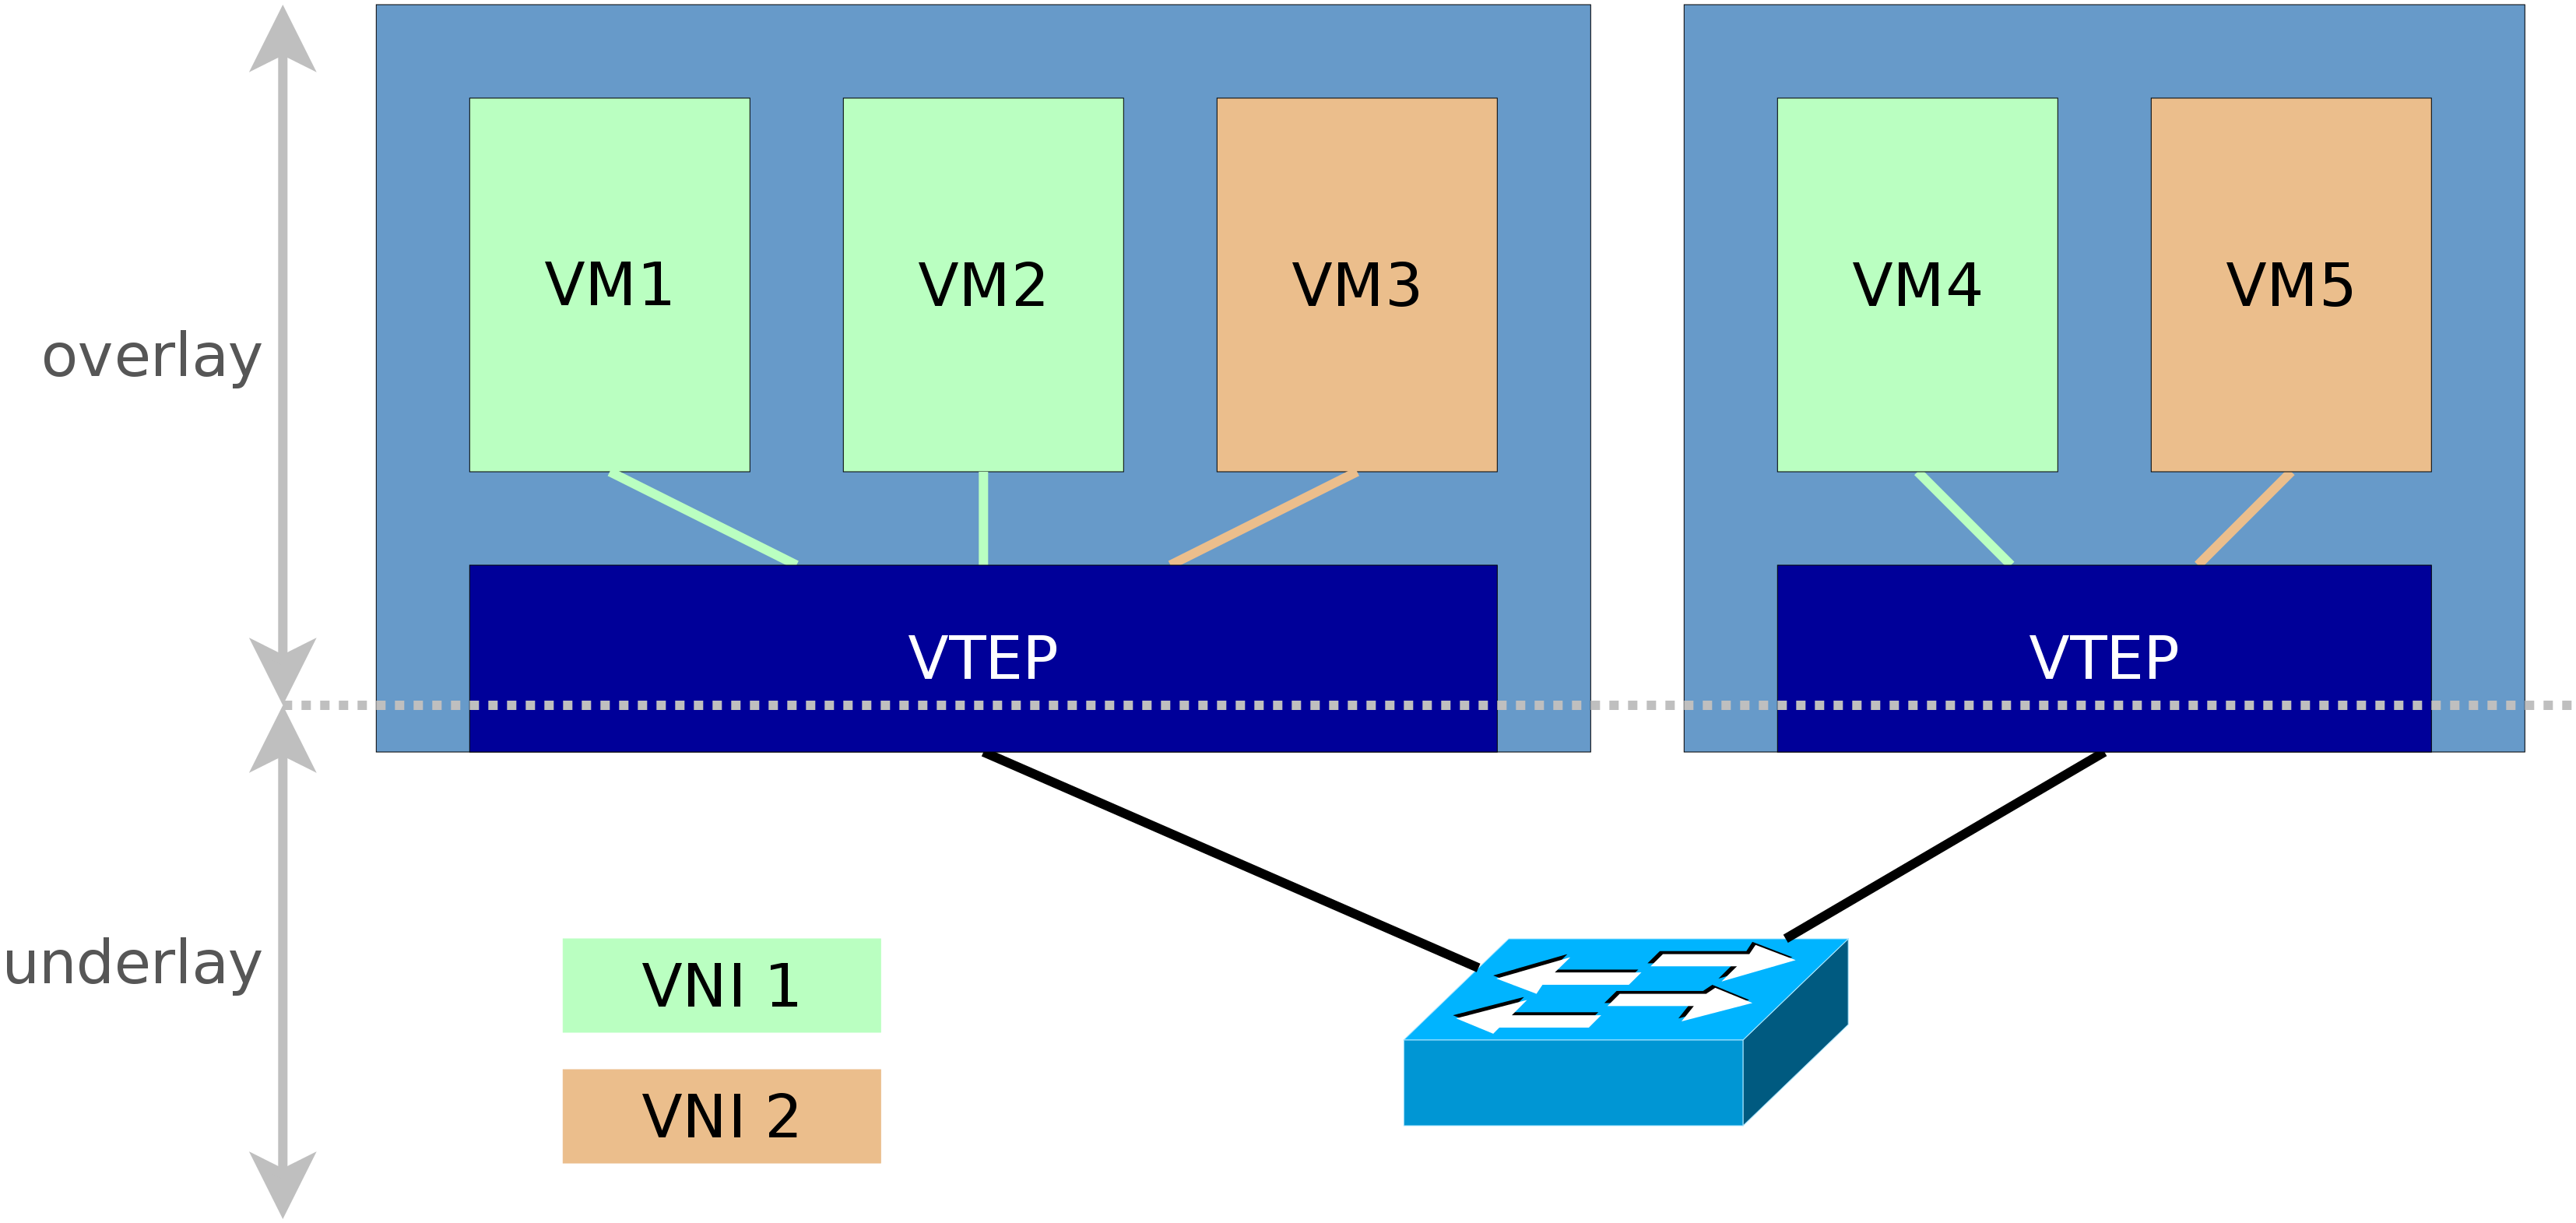
\includegraphics[width=0.9\textwidth]{vxlan.png}
	\end{center}
	\caption{Model of VXLAN topology}
	\label{img:vxlan-topology}
\end{figure}

\subsubsection{NVGRE}
Network virtualization using \Ac{GRE} is another overlay technology for multi-tenant data centers. It is very similar to previously mentioned \Ac{VXLAN} because it uses same topology scheme with different encapsulation mechanism. I am not going to provide detailed description of protocol as with \Ac{VXLAN} but main differences will be mentioned. Further information and current draft version can be found in \cite{draft-nvgre}\cite{rfc2748}\cite{rfc2890}.

The biggest difference is encapsulation mechanism. \Ac{VXLAN} uses special approach but \Ac{NVGRE} uses \Ac{GRE}.  Using quite old encapsulation standard may be beneficial because some boxes already support it and there is no need to make significant changes to physical infrastructure. Details about encapsulation mechanism can be found in \cite{rfc2748} and \cite{rfc2890} describes header extensions used to carry \Ac{VSID}. \Ac{VSID} is identifier for virtual subnet isolation, it is analogue of \Ac{VNI} used by \Ac{VXLAN} with same length of $24~\Jed{b}$.

Outer packer header with encapsulated payload is sent to destination \Ac{NVE} thus usage of \Ac{ECMP} may be suboptimal. There may be lack of entropy in outer header because destination address is same for all virtual machines residing at same \Ac{NVE}. This problem can be solved in \Ac{ECMP} hashing procedure by integrating \Ac{VSID} into sources for hash generation.

Multicast and broadcast traffic within overlay network is handled using multicast in underlay network. There is also defined N-Way unicast which do not depend on multicast: "In N-Way unicast, the sender NVE would send one encapsulated packet to every NVE in the virtual subnet. The sender NVE can encapsulate and send the packet as described in the Unicast Traffic Section 4.3. This alleviates the need for multicast support in the physical network." \cite{draft-nvgre}
However, this solution is suboptimal because there is unwanted packet duplication and thus it is better to deploy multicast and use it as a carrier mechanism.

\Ac{NVGRE} definition \cite{draft-nvgre} is still labeled as a draft, last version was published on 2014-11-05 and new updates are expected. Proposed draft is  simple and there are still mayor problems waiting to be solved. For example there is not any method how to distribute locations of addresses within overlay network. Document \cite{draft-nvgre} says: "This information can be provisioned via a management plane, or obtained via a combination of control plane distribution or data plane learning approaches. This document assumes that the location information, including VSID, is available to the NVGRE endpoint." It is obvious that this need to be solved before deployment in production use. 

\subsubsection{STT}
Last but not least technology used for building overlay network is Stateless Transport Tunneling (\Ac{STT}). It is designed to meet common requirements as allow overlapping of tenant's address space, decouple virtual network from physical infrastructure and to allow an unlimited virtual machine migration.

Basic principle is still same - some box (usually called \Ac{NVE}) encapsulates packets from overlay network and send it through underlay network to other \Ac{NVE}s. However, \Ac{STT} introduces completely new encapsulation method. \Ac{TCP}-like header is used as an encapsulation header but there is no three-way handshake or sessions because packets are processed different way. Header is used only as a storage for metadata about encapsulation. Field called Context Identifier is assigned to every flow and it is used as a generalized form of virtual network identifier. \cite{draft-stt} It is beneficial to use this generalization because there is space for future services. Space reserved for Context Identifier is 64 bits long so there is really enormouns amount of combinations available.

It is important for every overlay technology to support \Ac{ECMP} because efficient flow distribution between multiple paths can be used for underlay network in data center. First important requirement is to route each packet belonging to single flow same way and it is accomplished by using same ports and addresses for these packets. 
Second requirement is to provide enough of entropy for uniform flow distribution. Packet's source port is function of inner header and thus it provides entropy data for \Ac{ECMP} mechanism.

Using almost standard \Ac{TCP} segmentation for encapsulation is advantageous because it may bring significant performance improvement. Segmentation offloading is heavily used these days and it can be used to speed-up encapsulation process. The most important advantage of \Ac{STT} is providing new functions and using existent hardware techniques.

However, I can see some problems with deploying \Ac{STT}. First and the most important is changing meaning of \Ac{TCP} header field since this will probably cause problems in middle boxes. It is necessary to adjust configuration of state firewalls to allow \Ac{STT} because \Ac{TCP} headers are expected to behave different. Defining document \cite{draft-stt} is still in a draft version and it is already expired. Last version is \#06 at time of writing this paragraph (2014-11-13) and this version expired on 2014-10-17. It is possible that this technology will be used in the future but I do not think it is going to be used as overlay technology very often these days.

\subsection{Hop-by-hop network virtualization}
It is possible to use new technologies, e.g. \Ac{SDN}, and build different kind of virtual network called hop-by-hop. Hop-by-hop virtual network is totally different than previously described overlays since it does not use any encapsulation and data path is established by joining independent links between hops.

Hop is responsible only for forwarding data unit to next hop and whole flow is directed by a controller. Controller is software appliance responsible for communication with physical boxes, distributing routes and analyzing packets received from forwarding plane. It is usually tightly collaborating with orchestrator.

There is different perspective on network since control plane is separated from forwarding plane and physical devices are used for fast packet transfers and data plane is responsible for network control. Every decision is performed in controller or orchestrator and propagated to forwarding plane through data plane. It is obvious that the orchestrator should not be physically centralized because it would create single point of failure so it is better to use any distributed solution.

%Hop-by-hop networks are tightly connected with topic called Software defined networking described in \ref{par:sdn}.

\begin{figure}[htb]
	\begin{center}
	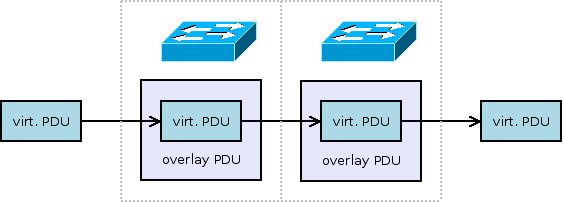
\includegraphics[width=0.9\textwidth]{overlay.png}
	\end{center}
	\caption{Overlay virtual network}
	\label{img:overlay}
\end{figure}


\begin{figure}[htb]
	\begin{center}
	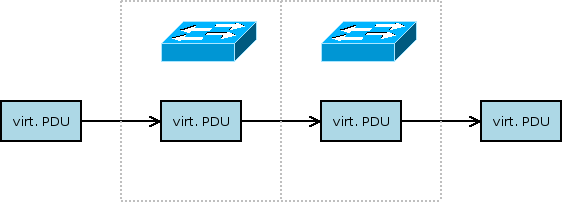
\includegraphics[width=0.9\textwidth]{hop-by-hop.png}
	\end{center}
	\caption{Hop-by-hop virtual network}
	\label{img:hop-by-hop}
\end{figure}

\subsection{Load balancing and high availability}
% load balancing

Load balancing is an essential part of service operation because it is required to achieve better scalability and availability than single machine approach can ever achieve. It is quite common in the past that one service had been served just by single machine. However, this solution is suboptimal since it is absolutely unscalable and it is impossible to provide high-availability solution.

It is necessary to employ service load balancing because load and service demand is still increasing and only properly designed load balancing solution can meet all of the requirements. Common requirements are
	\begin{itemize}
		\item low latency - request should be processed without any significant delay
		\item high availability - service should stay up during partial infrastructure failure
		\item scalability - infrastructure should be ready to increase resource when the load is enormous
	\end{itemize}

There are many different ways how to deploy load balancing and they differ by flexibility and functions available. We can be say that load balancing performed at higher levels is more flexible, but the best solution is a combination between two or more technologies on different layers. Appropriate solution depends also on access method because there are different balancing possibilities for \Ac{HTTP} \Ac{API}, remote terminal service and video streaming service. Methods presented in the following text will be general as well as access method specific, right use case will be always mentioned.

% scale-up / scale-out
Load balancing is closely related with scaling. There are two types of scaling - scaling-up and scaling-out. Scaling-up is accomplished by using more powerful resources, e.g. using interfaces with higher line rate or upgrading the server. It is easier, achievable faster and does not require load balancing, but it is quite easy to reach limit of scaling-up. 1G Ethernet \Ac{NIC}s are very common, 10G are a bit more expensive but still possible to buy and 100G are very rare and extra expensive. It is also necessary to take economical aspect into account since performance improvement and price function are not equally steep. 

Scaling-out is other possible scaling schema and it is accomplished by adding many parallel workers with common capacity. This approach is more favourable from economical view because performance growth is almost linear and technical benefit lies in redundancy. However, it is necessary to use load balancing to distribute workload across nodes. I think that the best scaling solution lies somewhere between so I would recommend to slowly scale-up and use scale-out for massive increase of performance.

% session persistance
Load balancing methods can be divided into two groups by session persistence. Session persistence mean that one client is always routed to same computing node. It is required if there is a client's information, called session, available only on this computing node and session would be lost in case of redirecting to another node. Application can be designed with taking load balancing into account and thus it does not require session persistence. However, session persistence is usually needed for load balancing of the services designed without load balancing capabilities.

\subsubsection{DNS based approach}
\Ac{DNS} load balancing is the first possible solution because it takes place before establishing session between a client and the server. It is relative easy to deploy and application redesign may not be necessary. Basic implementation can be, for example, round-robin \Ac{DNS} which is carried out by assigning many AAAA or A records for service host name. Client selects one record during resolving host name and use it thus basically performs load balancing already at user's device. This method is really simple but it lacks any advanced management options. First problem is with high availability because it is not possible to quickly remove host from a zone in case case of a failure. There is a field called \Ac{TTL} assigned to every record in the zone and this field defines how long can be this record cached, maximum time between change in zone and propagation to all clients should be \Ac{TTL} a \Ac{SOA}. However, there are Internet Service Providers ignoring this standard so it is possible that some client will still get wrong records even after \Ac{TTL} expiration. Sample zone file with AAAA and A records and \Ac{TTL} 6 minutes is in figure \ref{code:zone}.

More advance variant of \Ac{DNS} based load balancing is modification of the zone performed by an authoritative \Ac{DNS} server. There is usually just one AAAA/A record for service hostname, but returned \Ac{IP} address can be different for each query. This method can use geolocation and return \Ac{IP} address of the nearest server according to user's position, although user can use different recursive servers and geolocation can be very inaccurate. Technically this method is only variation of previously mentioned with better control of distribution and the problem with \Ac{TTL} is still remaining. This method is used by web portal Seznam.cz for load balancing between primary and secondary data center. They use \Ac{TTL} 5 minutes and also experienced problem with incorrect caching but I am not allowed to publish any detailed information.

Another problem with DNS load balancing, especially failover, is \Ac{DNS} pinning. It is mechanism implemented in web browsers to make \Ac{DNS} rebinding attacks more difficult. This attack is based on the pushing faked \Ac{DNS} record to client and then forward all traffic to attacker's \Ac{IP} address. Browser with pinning implemented \Uv{pins} first resolved \Ac{IP} address and use it even after \Ac{TTL} expiration so it basically prevents load balancing mechanism from switch client to another computing node. Further information can be found in \cite{dns-pinning}.

\begin{figure}[htb]
\caption{Example zone file for DNS load balancing}
\label{code:zone}
\begin{verbatimtab}
app.example.com	360	IN	AAAA	2001:db8::1
app.example.com	360	IN	AAAA	2001:db8::2
app.example.com	360	IN	AAAA	2001:db8::3
app.example.com	360	IN	A	192.0.2.1
app.example.com	360	IN	A	192.0.2.2
app.example.com	360	IN	A	192.0.2.3
\end{verbatimtab}
\end{figure}

\subsubsection{Application level load balancing}
One of the most flexible method is application load balancing. Is is performed on Layer 7 so it is possible to differentiate all lower layers. This solution is beneficial because application is able to decide on exact mapping between the customer connection and the working node. 
Customer is connected to balancing part of an application at first. This part (group of nodes) is responsible for the redirecting or forwarding request to a computing node. Login can be required before redirection and then the request if forwarded according to information acquired during login. Every information about the customer is already available, like ans \Ac{IP} address and login name, so computing node can be selected and it is also very simple to achieve session persistence. Balancing procedure is depicted in the figure \ref{img:balancing-application}.

Advantage of this method is direct connection between client and computing node, so balancing part is not overloaded with forwarding requests between users and computing nodes. Direct connection eliminates bottlenecks because there is not any central authority responsible for load balancing. Technically there is a central authority in load balancing part, but it can be redundant and balanced using other method, e.g. \Ac{DNS} load balancing.  However, it is necessary to expose computing nodes to users network and thus some may say that is insecure. I think that exposing computing nodes to outside word is not security hazard because security should be provided by proper application design and network security. Obscurity is not good security approach, in my opinion.

\begin{figure}[htb]
	\begin{center}
	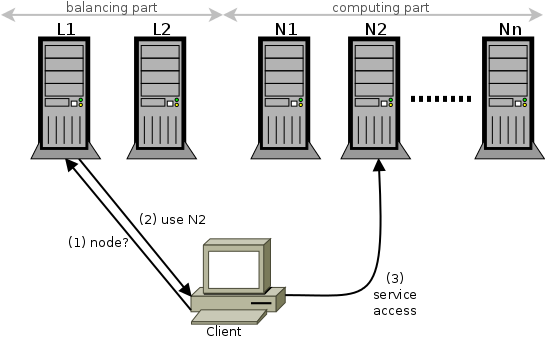
\includegraphics[width=0.9\textwidth]{balancing-application.png}
	\end{center}
	\caption{Load balancing at application level}
	\label{img:balancing-application}
\end{figure}

\subsubsection{Anycast load balancing}
It is possible to use anycast routing for load balancing and distribute workload between nodes. Typical architecture is depicted in the figure \ref{img:anycast-balancing} Only anycast \Ac{IP} address is propagated to outside world, so every incoming packet go to this destination address. This address is also assigned to local interfaces of compute nodes and advertised to local router using any routing protocol, e.g. \Ac{OSPF}. 

An incoming packet is delivered to local router and this router performs lookup and selects destination address according to it's actual routing table. This is advantageous because it is possible to assign priority to routes propagated by computing nodes and failed node is almost immediately removed from routing table.

However, this solution does not provide session persistence because packet can be routed to different computing node each time. There is a bottleneck in topology described in figure \ref{img:anycast-balancing} but this method can be adjusted to eliminate this problem and propagate different anycast addresses from different autonomous systems.

Global pool of root \Ac{DNS} servers use exactly this load balancing principle so request should always be delivered to the nearest server and thus almost perfectly distributed around world servers. According to data published in \cite{dns-anycast} up to 80\% of \Ac{DNS} queries are routed to the nearest anycast instance.

\begin{figure}[htb]
	\begin{center}
	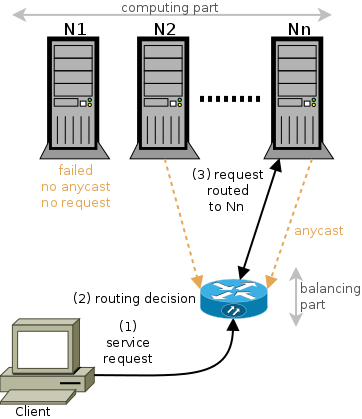
\includegraphics[width=0.7\textwidth]{balancing-anycast.png}
	\end{center}
	\caption{Anycast load balancing}
	\label{img:anycast-balancing}
\end{figure}

\subsection{Load balancers}
Load balancing of \Ac{TCP} flows can be performed on the network layer using box called load balancer. It does not have to be strictly physical box since there are also software solutions. This box modifies headers and basically translate flows from customer's side to internal and back. 

The simplest solution is rewriting destination address. Packet received on external interface of load balancer is analyzed, destination address is changed to one of the computation nodes and packet is delivered to computation node. Address rewriting must be performed also on packets received from computing node as well as on every related packet. 

Load balancer box must maintain a list of available computing nodes and continuously monitor their status because it have to select suitable node for every incoming flow. Monitoring method and node choosing algorithm depends on the application. It is also possible to integrate monitoring service into orchestrator and then control load balancer with an orchestrator.

It would be probably required to guarantee the session persistence so a load balancer will have to keep mapping table between customers and computing nodes. This table provides information about the current mappings and thus make it possible to deliver all packets from single flow to the same computing node.

Additional technologies can be integrated in the load balancer box, for example offloading, deep packet inspection or intrusion prevention. \Ac{SSL} offloading is used sometimes to decouple encryption from application running on computing nodes and to enable header rewriting. It is also possible to terminate \Ac{TCP} session on load balancer and establish new session for communication with computing node with maintaining packet's payload. It is even possible to carry out translation between \Ac{IPv6} and \Ac{IPv6}.

Load balancer box provides advanced function but is introduce bottleneck and single point of failure. Rewriting of packet headers and maintaining mapping table are even more resource expensive than router described in anycast load balancing. This solution is suitable for legacy application without any load balancing capabilities. 

%\subsection{Firewall}
% firewall 


%\subsection{Software Defined Networks}
%\label{par:sdn}
